\chapter{Optimal Dynamic Selection of Gear-ratios}  % to exploit or attenuate the external load dynamics
\label{sec:ControlAndPlanningOfRobotUsingVariableGearRatioActuators}

%\begin{flushright}
%\textit{"With four parameters I can fit an elephant, and with five I can make him wiggle his trunk."} \\ \emph{John von Neumann}
%\end{flushright}

\begin{flushright}
\textit{"He will win who knows when to fight and when not to fight."} \\ \emph{Sun Tzu}
\end{flushright}


The transmission gear-ratio that couples an actuator to a load has a significant effect upon the behavior of the actuator-load system. With a large reduction ratio, the load-side dynamics has no significant effect because it is attenuated by the factor of the square of the gear ratio. The net load acting on the actuator is mostly its own intrinsic load, including rotor inertia and friction. In contrast, with a small reduction ratio or a direct drive system \cite{asada_direct-drive_1987}, the behavior is usually dominated by the load-side dynamics which consist of highly non-linear inertial and gravitational forces for robotics manipulators. Sometime it can be advantageous to exploit the load-side dynamics: gravity may push the robot in a desired direction, dissipative torques induced on the actuator side may be small despite high-speed motion on the load side, etc. In other situations, however, it may be advantageous to be isolated from the load-side dynamics and external disturbances. For example, bearing a large load or moving it slowly against gravity requires a large reduction ratio.

This paper aims to explore the potentials of the actuator transmissions that can be switched dynamically to either attenuate or leverage the natural dynamics of the system. In section \ref{sec:princ}, the principle of load leveraging and attenuation is delineated for a simple 1-DoF manipulator, section \ref{sec:app} will discuss how this principle can be exploited in various applications, where bi-polar load conditions must be dealt with despite actuator weight and power constraints, and section \ref{sec:chal} will discuss related works. Section \ref{sec:ctl} will introduce a formal mathematical representation and propose control algorithms to automatically select optimal gear-ratios for a single DoF and multi-DoF systems. The advantage of actively changing the gear-ratio are illustrated with simulated experiments in section \ref{sec:sim} and with experiments with a custom robotic arm in section \ref{sec:ev}.

\subsection{Illustration of the principle for a 1-DoF manipulator}
\label{sec:princ}

Fig. \ref{fig:bigpicture} illustrates a simplified 1-DoF robotic manipulator where an electric motor is coupled to a pendulum through a gearbox with a gear-ratio $R$.

\begin{figure}[H]
 \vspace{-10pt}
	\centering
		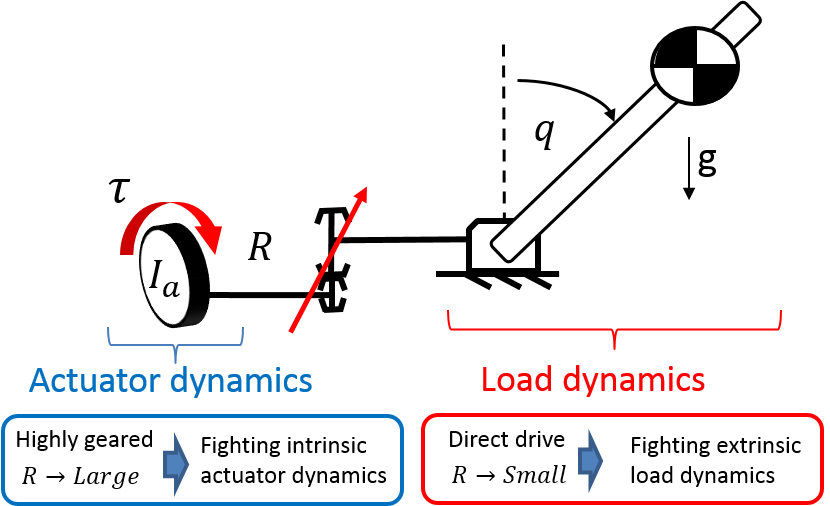
\includegraphics[width=0.75\textwidth]{bigpicture.png}
	\caption{Effect of the gear ratio on the dynamics}
	\vspace{-10pt}
	\label{fig:bigpicture}
\end{figure}

As illustrated by phase portraits in Fig. \ref{fig:pp}, if $R$ is small then the dynamic behavior of the system is dominated by the non-linear pendulum dynamics (Fig. \ref{fig:pp1}), but if $R$ is very large, the behavior is dominated by the intrinsic inertia of the actuator, leading to the double-integrator behavior (Fig. \ref{fig:pp2}).

\begin{figure}[H]
				\vspace{-10pt}
        \centering
				\subfloat[ Reduction ratio $R$=1 ]{ %extrinsic dynamics
				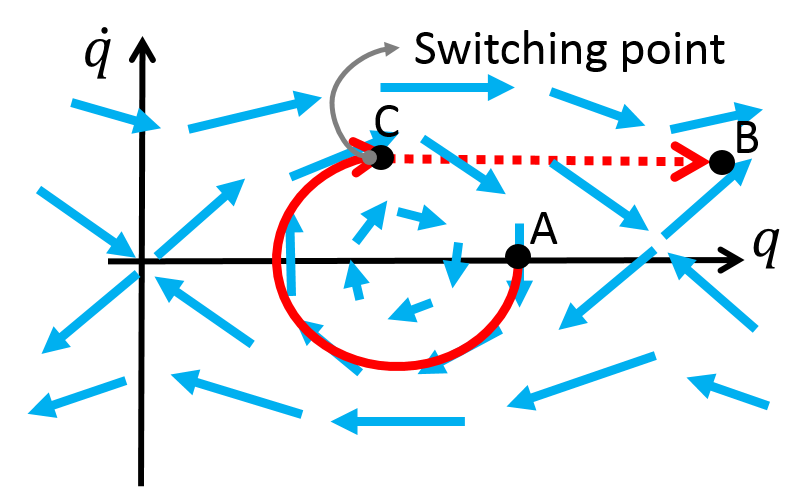
\includegraphics[width=0.40\textwidth]{pp1_hand.png}
				\label{fig:pp1}}
        \subfloat[Reduction ratio $R$=10 ]{ % intrinsic dynamics
				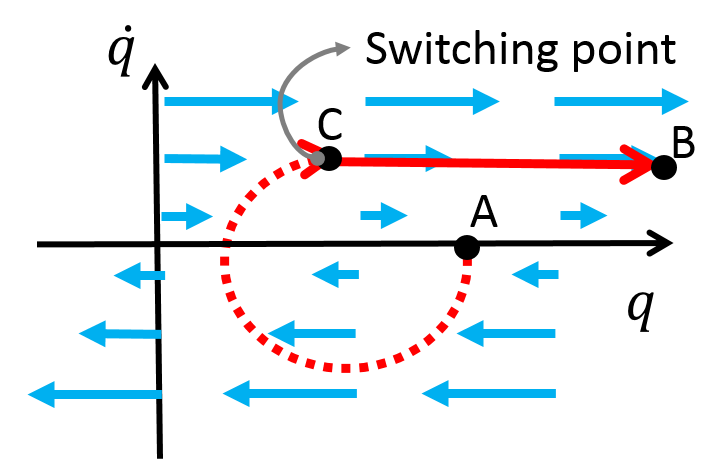
\includegraphics[width=0.40\textwidth]{pp10_hand.png}
				\label{fig:pp2}}
        \caption{Phase portraits illustrating the dynamical behavior}
				\label{fig:pp}
\end{figure}

The vector fields of Fig. \ref{fig:pp} illustrate the evolution of the system with no actuator torque. Suppose that we want to move from state A to state B on the phase plane. Starting off state A with the gear-ratio of 1:1 brings the system along the curved trajectory shown in Fig. \ref{fig:pp1}. Switching the gear ratio at state C to 1:10 will change the trajectory to the one in Fig. \ref{fig:pp2}, and bring the system to the destination state B. Note that no actuator torque is necessary for following this trajectory. A salient feature of actively changing the gear-ratio is that a vector field having properties useful for moving in a desired direction can be selected to minimize the necessary torque to apply to the system. 


\subsection{Challenges and related works}
\label{sec:chal}

This paper investigates the control of robots with variable gear-ratio actuators. This differs from variable stiffness actuators that use a variable transmission placed between a compliant element and the load \cite{vanderborght_variable_2013}, where it influence the reflected output stiffness but not the steady-state power transmission characteristics. While variable gear-ratio actuators have been studied extensively for automobile power-trains, they have not yet been fully investigated in robotics, despite significant potential gains. Variable gear-ratio transmissions for electric motors have been proposed for legged locomotion \cite{hirose_design_1991}, grasping robotic hands \cite{shin_robot_2012} , propulsion system \cite{lee_new_2012} \cite{mckeegan_antonovs_2011} and actuation systems \cite{girard_two-speed_2015} \cite{hirose_development_1999} \cite{tahara_high-backdrivable_2011}. Some of those works address the issue of how to change the gear-ratio, but there is no general approach to the high-level control of automatically selecting the right gear-ratio for nonlinear, coupled multi-DoF robotic systems.


From the control perspective, automating the gear-ratio selection in a robotic context is a new and challenging problem. Gear-shifting is a very non-linear process and the plant becomes a hybrid dynamical system if the usable gear-ratios are a set of discrete values. In simple scenarios, the gear-ratio selection can be based on simple principles. For instance, for a system running at a steady speed, the best gear-ratio can be selected based on efficiency. Alternatively, for rapid acceleration, the gear-ratio may be selected based on the actuator-load inertia matching \cite{giberti_effects_2010} \cite{chen_generalized_1991}. A multi-DoF robot, however, experiences diverse types of forces acting simultaneously. These include gravity, friction, and inertial forces as well as Coriolis and centrifugal forces. Hence, it is challenging to find a general control policy for selecting gear-ratios for the multitude of dynamically interacting actuators in the robotics context. Mixed-integer programming has been used to generate optimal open-loop trajectories of complex dynamical system with both continuous torque and discrete gear-selection input variables \cite{gerdts_solving_2005}. However, open-loop trajectories can be unstable and new trajectories must be computed for each initial goal and target pair. Dynamic programming was used to generate feedback laws for torque and gear-ratio selection in simple systems \cite{girard_practical_2016}. However, this technique is computationally expensive, it does not scale well to high-dimensional systems, and it required a significant amount of offline computation for each different goal position. Here in this paper, a model-based approach is proposed, with the advantage of scaling to high-dimensional robotics system. The method is applied to trajectory tracking, and the entire trajectory and gear-ratio control law is synthesized so that small actuators can dynamically lift a heavy load. The focus will be on systems where the gear-ratio options are limited to a discrete set, but the proposed principle and control algorithms are also applicable to robots with continuously variable transmissions.


\section{Modeling}
\label{sec:model}

\begin{flushright}
\textit{"With four parameters I can fit an elephant, and with five I can make him wiggle his trunk."} \\ \emph{John von Neumann}
\end{flushright}


Variable gear-ratios can be modeled as variable transformer elements, using the bond-graph terminology. This representation provides a clear physical understanding of the effect of gear-ratio even in a non-linear multi-DoF system. Furthermore, this modeling approach facilitates the implementation of a real-time optimization in the proposed controller. Limitations are discussed at section \ref{sec:limitation}.

\begin{table}[htbp]
	\centering
		\begin{tabular}{ c c l }
		
        \hline \hline
			$H$             &  :  & External inertia matrix \\
			$D$             &  :  & External damping matrix \\
			$C$             &  :  & External Coriolis/Centrifugal forces matrix  \\
			$\vec{f}_g$     &  :  & External gravitational forces vector  \\
			$\vec{d  }$     &  :  & External disturbances forces vector  \\
			$R$             &  :  & Gear-ratio matrix (diagonal) \\
			$I$             &  :  & Intrinsic actuator inertia matrix (diagonal) \\
			$B$             &  :  & Intrinsic actuator damping matrix (diagonal) \\
			$\vec{\tau}$    &  :  & Electromagnetic motor torques  \\
			$\vec{q}$       &  :  & Joint coordinates position vector  \\
			$\vec{w}$       &  :  & Actuator coordinates velocity vector  \\
			$J$             &  :  & task-space coordinates / joint coordinates jacobian matrix\\
			%&\text{Secondary variables:  \\
			$\vec{f}$       &  :  & Net transmitted forces (joint coordinates) \\
			$\vec{\tau}'$   &  :  & Net transmitted forces (actuators coordinates) \\
			$\vec{\tau}_I$  &  :  & Sum of intrinsic forces  \\
			$\vec{\tau}_E$  &  :  & Sum of extrinsic forces  \\
		\hline \hline
        \end{tabular}		
        \caption{Nomenclature}	% Table caption must be placed on top of the table %
		
	\label{tab:nom}
\end{table}

\subsubsection{1-DoF system}
\label{sec:1DOFSystem}

Fig. \ref{fig:bondgraph1} shows the bond graph model of the 1-DoF robot in Fig. \ref{fig:bigpicture}, including dissipative forces.

\begin{figure}[htp]
	\centering
		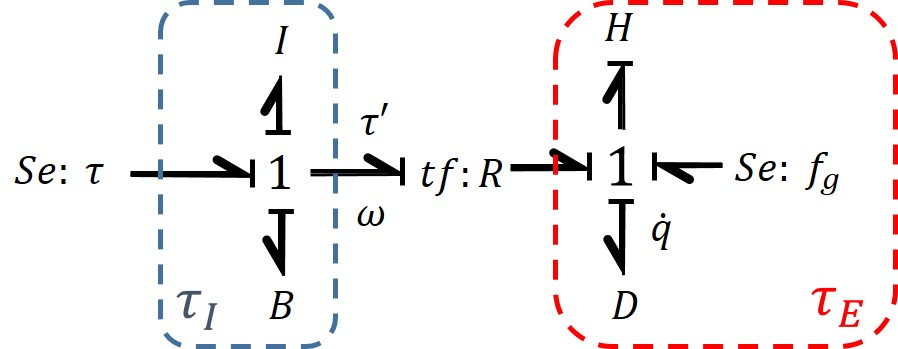
\includegraphics[width=0.60\textwidth]{bondgraph1.jpg}
	\caption{Model of a 1-DoF robot with a variable gear-ratio actuator}
	\label{fig:bondgraph1}
\end{figure}

If the actuator's intrinsic resistive forces $\tau_I$ are approximated to a linear quantity, the equations of motion (EoM) can be written as:
%
\begin{align}
	\underbrace{\left[	H \ddot{q} + D \dot{q} + mg\sin( q )	\right]}_{\tau_{E}(\ddot{q},\dot{q},q)}
	&= R \tau - R^2
	\underbrace{\left[ I \ddot{q} + B \dot{q}	\right]}_{\tau_{I}(\ddot{q},\dot{q})} \\
	\tau &= 	\frac{\tau_{E}(\ddot{q},\dot{q},q)}{R} + R \; \tau_{I}(\ddot{q},\dot{q})
	\label{eq:1dofEoM}
\end{align}
%
where the effect of the gear ratio can be seen clearly; increasing $R$ attenuates the external dynamic terms $\tau_{E}$ but amplify the intrinsic actuator losses $\tau_{I}$ for a given trajectory.

\subsubsection{Generalization to n-DoF manipulators}
\label{sec:GeneralizationToNDOFManipulators}

To generalize the above model to a $n$-DoF system with $n$ actuators, the load-side dynamics is considered as a generic form of manipulator equations where each port is connected to an independent actuator through a network of transformers. 
%
\begin{figure}[htp]
	\centering
		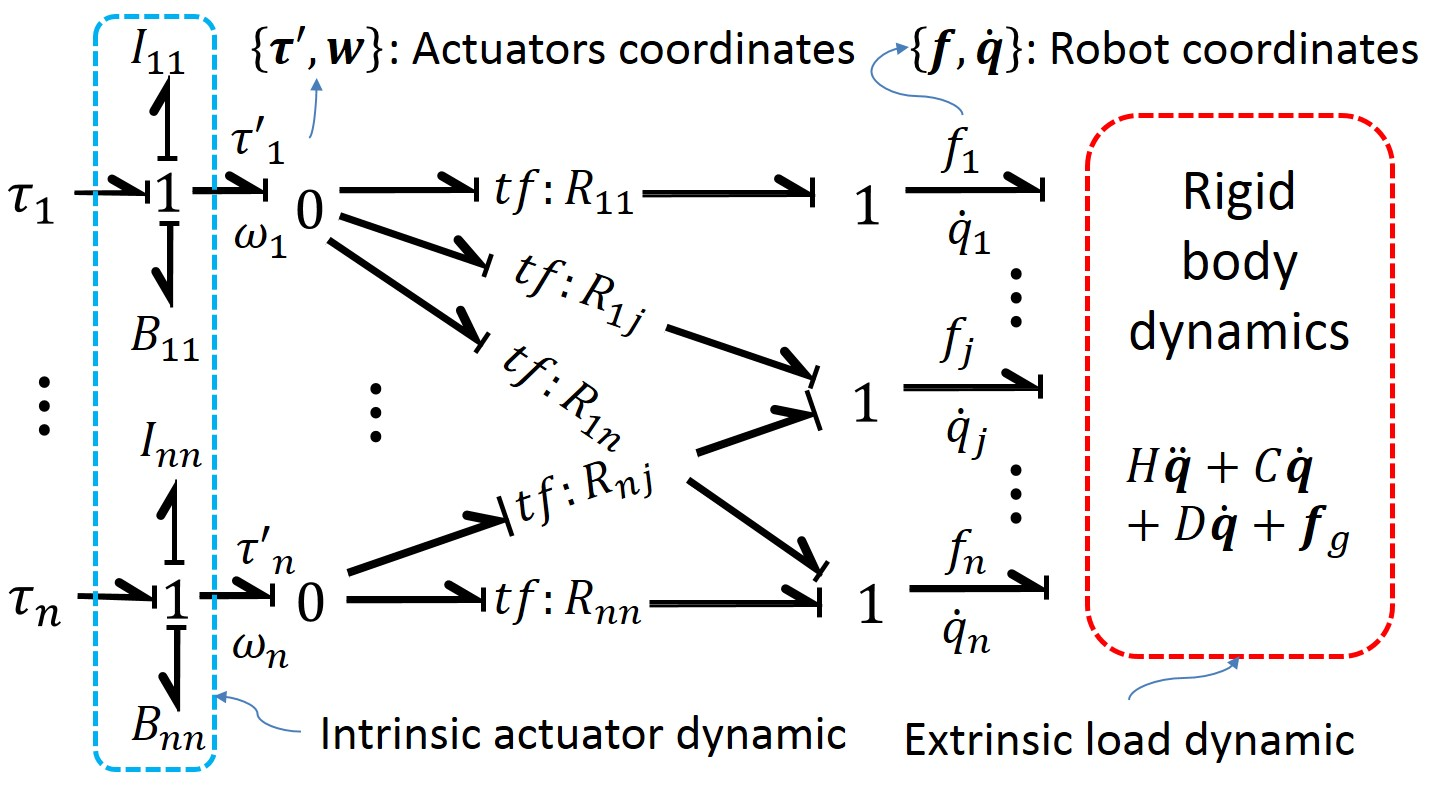
\includegraphics[width=0.70\textwidth]{bondgraph.jpg}
	\vspace{-10pt}
	\caption{Model of a $n$-Dof robot with variable actuator-joint coupling}
	\label{fig:bondgraph}
\end{figure}
%
The network of transformers can be view as a type of coordinate transformation relating effort (force or torque) and flow (velocity or angular velocity) on the load side ($\vec{f}$,$\dot{\vec{q}}$) to those on the actuator output side ($\vec{\tau}'$,$\vec{w}$):
%
\begin{align}
	\vec{ f } = R^T \vec{\tau}' \quad  \quad R \dot{ \vec{q} } = \vec{w}
 \label{eq:coortransform}
\end{align}
%
where $R$ is a $n$ by $n$ matrix consisting of all the transformer ratios. The EoM are then given by:
%
\begin{align}
	&\underbrace{ H \vec{ \ddot{q} } + C\vec{ \dot{q} } + D \vec{ \dot{q} } + \vec{ f }_g  + \vec{ d }}_{ \vec{\tau}_{E}(\ddot{\vec{q}},\dot{\vec{q}},\vec{q},\vec{d})}
		= R^T \underbrace{  \left[ 
		\vec{ \tau } - I \vec{ \dot{w} } - B \vec{ w }       
		\right]}_{ \vec{\tau}' } 
 \label{eq:eom_ndof}
\end{align}
%
Note that, in the case of locomotion or manipulation where the robot interacts with environment by physically contacting it, the dynamic model $\vec{\tau}_{E}$ must reflect the contact conditions, either by considering contact forces as known disturbances $\vec{ d }$ or by formulating $\vec{\tau}_{E}(\ddot{\vec{q}},\dot{\vec{q}},\vec{q})$ as a hybrid dynamical system. In the latter case, multiple dynamic equations associated with individual contact conditions must be constructed and used in real time.

In most practical cases, each actuator has its independent variable transmission and, thereby, the $R$ matrix will be diagonal and each diagonal value can be selected independently. Assuming this situation, the EoM can be simplified to a form, similar to the scalar case, illustrating the effect of the gear ratios matrix $R$: 
%
\begin{align}
	\vec{\tau} &= R^{-1} 
	\underbrace{ 
	\vec{\tau}_{E}(\ddot{\vec{q}},\dot{\vec{q}},\vec{q},\vec{d}) 
	}_{\text{External load dynamics}}
	+ R 
	\underbrace{ 
	\vec{\tau}_{I}(\ddot{\vec{q}},\dot{\vec{q}})
		}_{\text{Intrinsic losses}}
	\\ %&\text{where} \;
	\vec{\tau}_{I} &\triangleq I \vec{ \ddot{q} } + B \vec{ \dot{q} } 
	%[ \vec{\tau}_{I} ]_j &\triangleq [I]_{jj} [\vec{ \ddot{q} }]_j + [B]_{jj}  [ \vec{ \dot{q} }]_j  \quad \forall j \in {1,2,...,n}
 \label{eq:eom_ndof2}
\end{align}
%
\subsubsection{Limitation of the simplified model}
\label{sec:limitation}
%
The main assumption of the proposed model is that gear-ratios are considered as independent control inputs, neglecting all the dynamics and delays associated with the transition of gear ratio. Physically this implies that the kinetic energy of the system may be discontinuous at a gear-shift since the energy necessary for the transition is not considered. In the case of a car transmission, the engine speed is synchronized to the wheel speed before engaging the next gears. This model would not keep track of the energy used for accelerating or braking the engine during the synchronization process. This model can be used if the gear-shift process is fast compared to the dynamics of the robots and if the energetic losses due to the gear-shift are negligibly small. In addition this model also assumes that all motor rotors are in an inertial reference frame, neglecting gyroscopic effects, which may be induced when the axes of motor rotors are rotated.


\section{Model-based control approach}
\label{sec:HierachicalControlApproach}


\subsection{Optimal Gear ratio along a trajectory}

This section analyzes the optimal gear-ratio at each instant along a known trajectory. 

\subsubsection{Selection criteria}
\label{sec:GearSelectionCriteria}

The two main advantages of changing gear-ratio are 1) lowering the necessary torque to follow a trajectory and 2) modifying the effective impedance reflected on the environment. Optimization for reducing torque can be done by minimizing $\vec{\tau}^T \vec{\tau}$ at each point along the trajectory. Optimization for reflected impedance can be done by minimizing the difference between desired task-space impedance and the actual one, which is directly affected by the matrix $R$. For instance, the end-point inertia matrix contains the gear ratios: 
%
\begin{align}
	M = [J(\vec{q})^T]^{-1} \big [ \underbrace{ R^T I R }_{\text{Actuator contribution}} + H( \vec{q} ) \big ] J(\vec{q})^{-1}
 \label{eq:endpointmass}
\end{align}
%
Another point of practical importance is that the rotor speed should be constrained to be lower than their maximum velocity. This is to avoid infeasible gear shifts. For example, attempting to shift to a low gear at an extremely high speed is impossible. 

\subsubsection{Optimization}
 The optimal gear-ratio is determined by minimizing the total actuator torques and, optionally, the difference in end-point impedance:
%
\begin{align}
	R^{*}(\ddot{\vec{q}},\dot{\vec{q}},\vec{q},\vec{d}) &= \operatornamewithlimits{argmin}\limits_{R} \left[ \vec{\tau}^T \vec{\tau} + \alpha \| M_{d} - M \| \right]  \\
	& \text{s.t}  \quad R \dot{\vec{q}} \leq \vec{w}_{max} 
\label{eq:rmin_general}
\end{align}
%
where $\alpha$ is a parameter to set the trade-off between minimizing motor torques and matching the desired end-point inertia.
%
For a 1-DoF system, the optimal gear ratio leading to minimal torque, not considering any velocity constraints, at a given instant on a trajectory is given by

\begin{align}
	R^{*} &= \operatornamewithlimits{argmin}\limits_{R} \left[ \tau^2 \right] = \sqrt{ \left | \frac{\tau_{E}(\ddot{q},\dot{q},q,d)}{\tau_{I}(\ddot{q},\dot{q})} \right |   } 
\label{eq:aaa}
\end{align}

Similarly for a multi-DoF system, if $R$ is a diagonal matrix, the optimal gear-ratios can be obtained independently for each axis:
\begin{align}
	%R^{*} = \operatornamewithlimits{argmin}\limits_{R} \left[  \vec{\tau}^T \vec{\tau} \right] \Rightarrow 
	[R^*]_{ii} = \sqrt{ \left | \frac{ [\vec{\tau}_{E}(\ddot{\vec{q}},\dot{\vec{q}},\vec{q},\vec{d})]_i }{ [\vec{\tau}_{I}(\ddot{\vec{q}},\dot{\vec{q}})]_i } \right | }
 \label{eq:rmin2}
\end{align}

Note that large gravitational forces or external disturbances, only present in $\vec{\tau}_{E}$, will usually lead to larger optimal gear-ratios, unless they cancel-out other forces in a way that makes $\vec{\tau}_{E}$ smaller. If inertial or viscous forces, present both in $\vec{\tau}_{E}$ and $\vec{\tau}_{I}$, dominate, then the optimal gear-ratio will be a compromise such that extrinsic and intrinsic forces are balanced, a form of impedance matching. The optimal gear ratio given by \eqref{eq:rmin2} includes both gravity, inertial and viscous effects as well as all other effects, hence it can be applied to any arbitrary dynamic situations.

\newpage

\subsubsection{Examples}
\label{sec:Examples}

Here eq. \eqref{eq:aaa} is applied to the robot in Fig. \ref{fig:bigpicture} in simple scenarios. 

\paragraph{Acceleration from rest} 

When the robot accelerates from rest with no viscous forces, the optimal gear ratio at the up-right position, where no gravity acts, is given by:
\begin{align}
	R^{*}  = \sqrt{ \left | \frac{H \ddot{q} }{ I \ddot{q} } \right |   } = \sqrt{ \frac{H}{I}}
 \label{eq:impmatching}
\end{align}
In this situation, the problem is reduced to impedance matching for two inertial loads. The optimal gear ratio minimizing the torque for a given acceleration is the one for which the load inertia and the motor reflected inertia are the same.

\paragraph{Supporting gravity without moving}

In the situation where the robot is not moving and fighting against gravity, then the optimal gear ratio is:
\begin{align}
	R^{*}  = \sqrt{ \left | \frac{ f_g }{ 0 } \right |   } \rightarrow \infty
 \label{eq:gravrejection}
\end{align}
In this static case, the largest possible gear-ratio is the optimal choice. 


\subsubsection{Numerical Optimization}

If some of the assumptions used in the previous section are not valid or if the gear-ratios are limited to a few discrete choices, then the optimization must be computed numerically. The minimum needed is to have a model of the inverse dynamic, which could include any non-linearity, in the form:
\begin{align}
	\vec{\tau}  = f( \vec{\ddot{q}} , \vec{\dot{q}} , \vec{q} , \vec{d} , R ) 
\end{align}
In the situation of discrete gear-ratios, this lead to a combinatorial optimization problems, adding a constraint on the gear selection in the form of:
\begin{align}
	%R^{*} &= \operatornamewithlimits{argmin}\limits_{R} \left[  \vec{\tau}^T  \vec{\tau} + \alpha \| M_{d} - M \|  \right] \quad \\
	&  R \in \{R_1,R_2, ... , R_l\} 
\end{align}
However, if the number of options $l$ is reasonably small, then every possible options can be computed quickly. For instance, for the robot presented in this paper, see Fig. \ref{fig:arm_proto}, there is 3 actuators each with 2 gear-ratio options, leading to $l=2^3=8$ possible matrix $R$.



\subsection{Trajectory following controllers}

\subsubsection{R* Computed Torque}
\label{sec:RobustTrajectoryFollowingController}


The proposed closed-loop controller, shown in Fig. \ref{fig:bbb}, is based on the Computed Torque technique \cite{asada_robot_1986}, but includes an optimization step to compute and select the optimal gear-ratios. The idea is as follow, first compute a necessary acceleration $\ddot{\vec{q}}_r$ to guarantee convergence on the trajectory. Then given the actual position $\vec{q}$, actual speed $\dot{\vec{q}}$ and desired acceleration $\ddot{\vec{q}}_r$ compute the optimal gear-ratios $R^*$, as described previously for a known trajectory, and apply the corresponding necessary torques $\vec{\tau}^*$. As illustrated, the model-based estimation of extrinsic and intrinsic forces can optionally be improved by using a disturbance observer. The salient feature of the R* controller is that the optimal gear-ratio is selected based on state-feedback, i.e. even in situations not foreseen in the planner that generated the nominal trajectory. For instance, if a disturbance pushes the robot in a state where the robot faces a large gravitational force requiring a large gear-ratio, the controller will automatically select it. Similarly if facing a contact forces, if it is included in the model or estimated with a disturbance observer, the R* controller will automatically select the appropriate gear-ratio. Fig. \pageref{fig:dq} offer a graphical interpretation of the R* algorithm in the phase plane. 

\begin{figure*}[t]
	\centering
		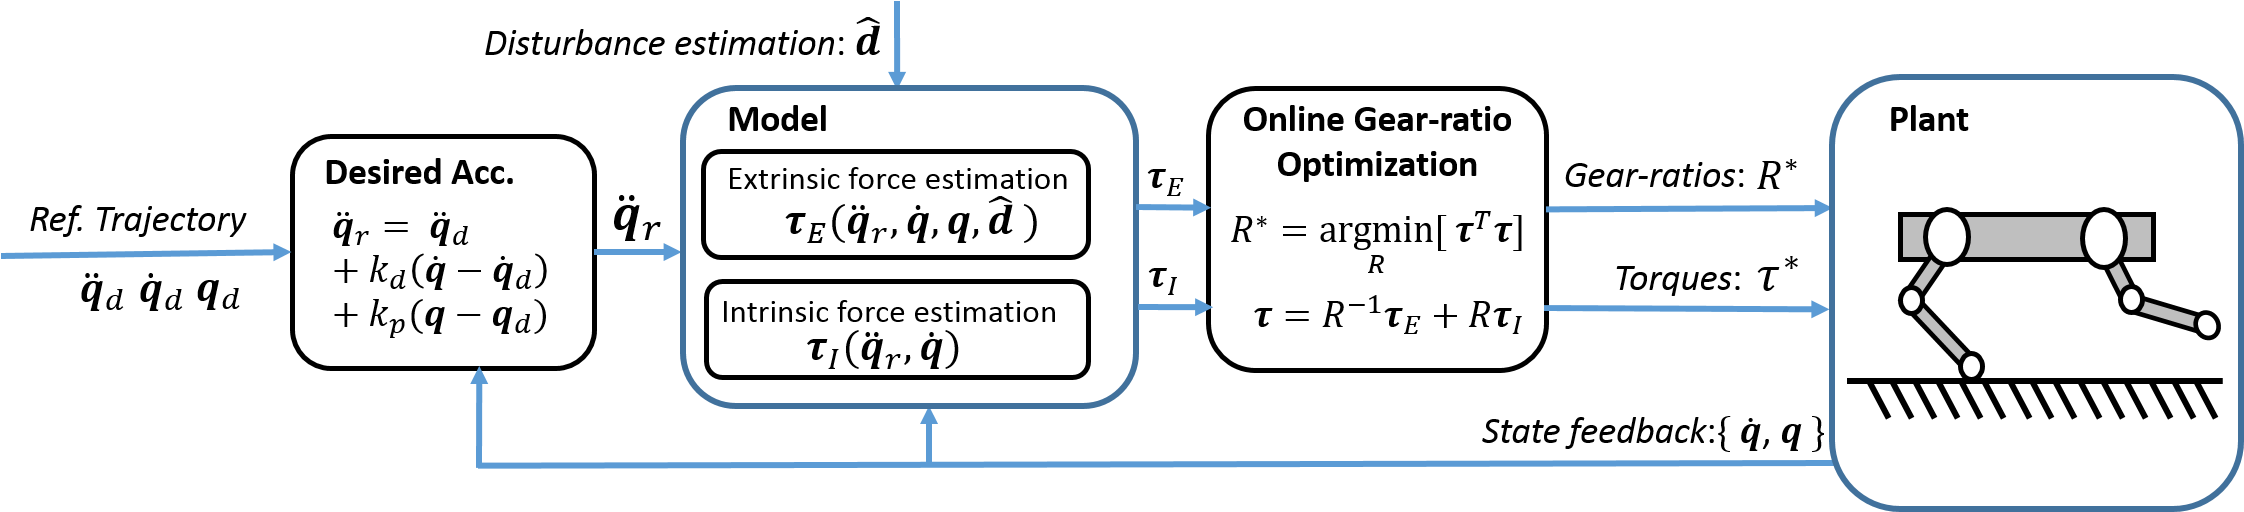
\includegraphics[width=0.95\textwidth]{Rstar_block_big.png}
	\caption{R* Computed Torque Controller}
	%\vspace{-10pts}
	\label{fig:bbb}
\end{figure*}

\begin{figure}[htp]
	\centering
		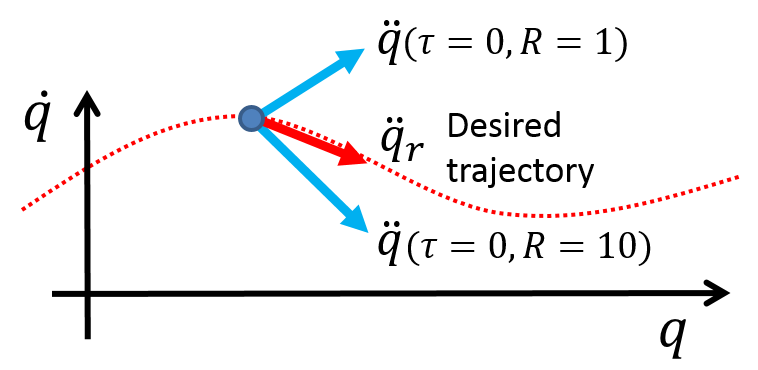
\includegraphics[width=0.40\textwidth]{dq.png}
	\caption{The R* algorithm can be interpreted graphically, as selecting the gear-ratio for which the natural acceleration vector is the closet to the desired acceleration vector $\vec{\ddot{q}}_r$ (after scaling the distance with the inertia), in order to minimize the necessary torques to apply on the system.}
	\label{fig:dq}
\end{figure}


\paragraph{Heuristic approach to minimize switching}

Because the control effort during gear-shifts is neglected in the model, using the proposed controller can lead to rapid switching between gear-ratios in certain situations. To avoid this undesirable behavior, it is proposed to add hysteresis to the controller: the gear-ratio is only changed if the difference of computed torque, between using the optimal and the previously selected gear-ratio, is greater than a minimum torque threshold, and also if the elapsed time since the last change is greater than a minimum delay. 

\subsubsection{R* Sliding Mode Controller}

\subsubsection{Heuristic approach to minimize gearshift}


\subsection{Trajectory planning}
\label{sec:SamplingBasedTrajectoryPlanner}


\section{Dynamic programming approach}
\label{sec:DynamicProgrammingAproach}



\begin{figure}[H]
	\centering
		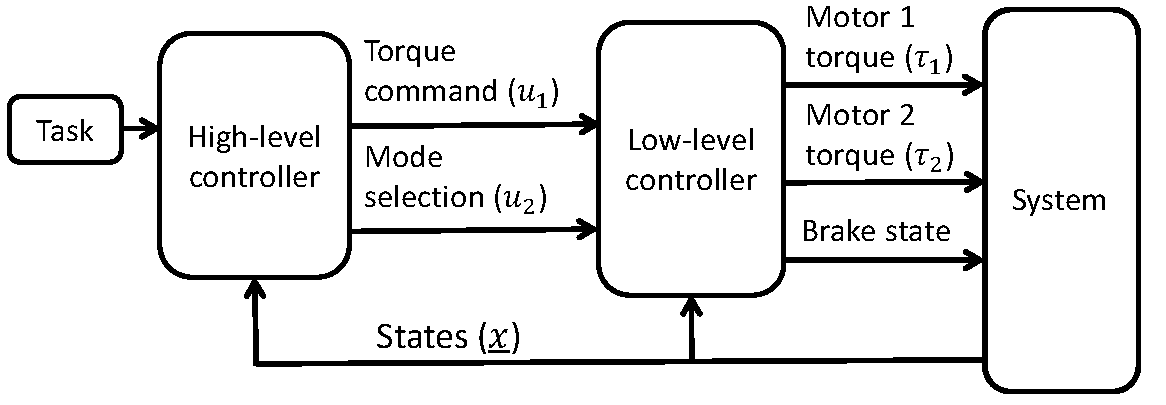
\includegraphics[width=0.45\textwidth]{blocks2.pdf}
	\caption{Controller architecture}
	\label{fig:blocks}
\end{figure}

\begin{figure}[H]
	\centering
		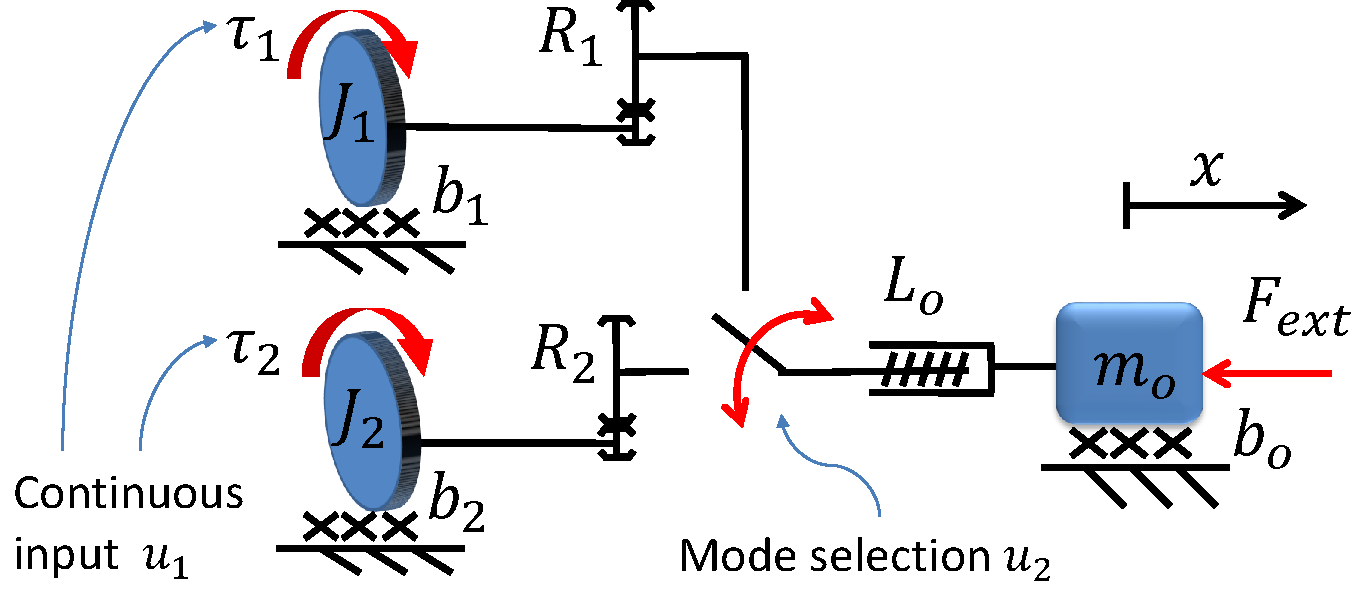
\includegraphics[width=0.42\textwidth]{model.pdf}
	\caption{Lumped parameter simplified model}
	\label{fig:model}
\end{figure}

\subsection{Value Iteration}


\begin{figure}[H]
        \centering
				\subfloat[Minimum time]{
        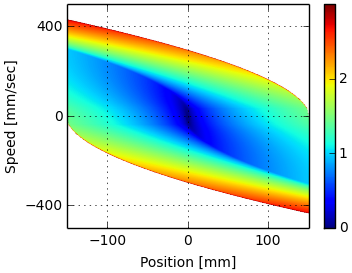
\includegraphics[width=0.32\textwidth]{Jt.png}
				\label{fig:J_time}}
        \subfloat[Quadratic cost]{
				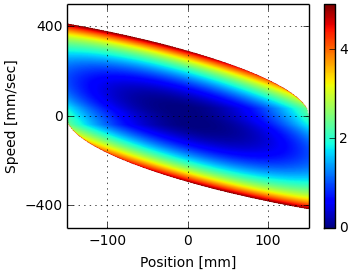
\includegraphics[width=0.32\textwidth]{Jq.png}%J_LQR.png
				\label{fig:J_LQR}}
				\subfloat[Minimum energy]{
				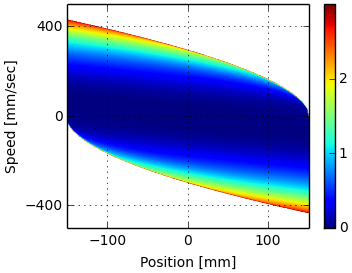
\includegraphics[width=0.32\textwidth]{Je.png}
				\label{fig:J_energy}}
        \caption{Optimal cost-to-go $J^*$}\label{fig:J}
\end{figure}

\begin{figure}[H]
        \centering
				\subfloat[Minimum time]{
        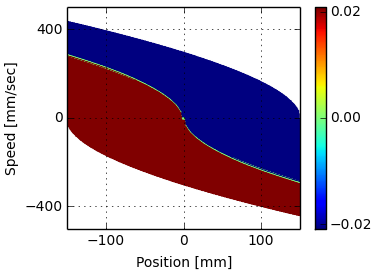
\includegraphics[width=0.32\textwidth]{u1t.png}
				\label{fig:u0_time}}
        \subfloat[Quadratic cost]{
				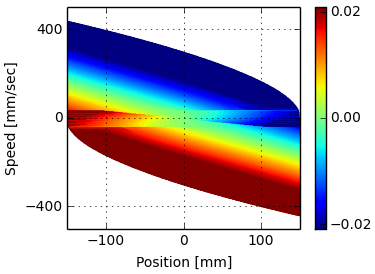
\includegraphics[width=0.32\textwidth]{u1q.png}
				\label{fig:u0_LQR}}
				\subfloat[Minimum energy]{
				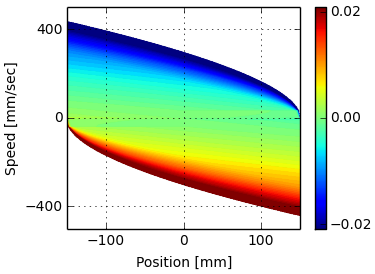
\includegraphics[width=0.32\textwidth]{u1e.png}
				\label{fig:u0_energy}}
        \caption{Optimal policy for the continuous torque command $u_1$ [Nm]}\label{fig:u0}
\end{figure}

\begin{figure}[H]
        \centering
				\subfloat[Minimum time]{
        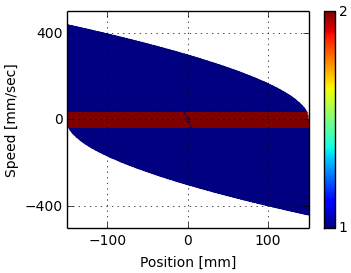
\includegraphics[width=0.32\textwidth]{u2t.png}
				\label{fig:u1_time}}
        \subfloat[Quadratic cost]{
				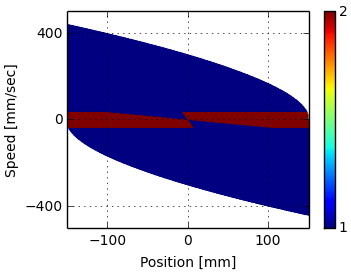
\includegraphics[width=0.32\textwidth]{u2q.png}
				\label{fig:u1_LQR}}
				\subfloat[Minimum energy]{
				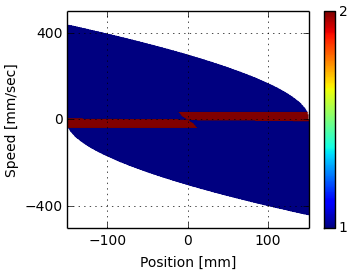
\includegraphics[width=0.32\textwidth]{u2e.png}
				\label{fig:u1_energy}}
        \caption{Optimal policy for the mode selection $u_2$}\label{fig:u1}
\end{figure}

\begin{figure}[H]
        \centering
				\subfloat[Minimum time]{
        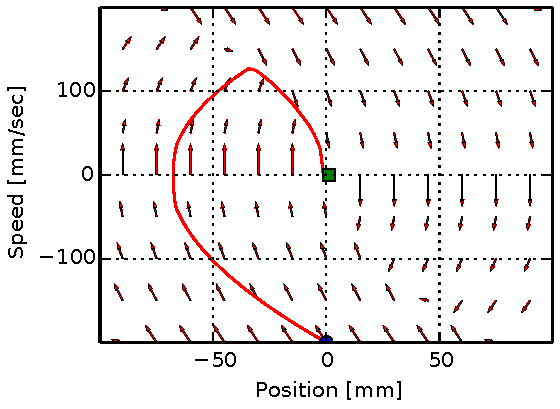
\includegraphics[width=0.32\textwidth]{ppt.pdf}
				\label{fig:phase_plane_time}}
        \subfloat[Quadratic cost]{
				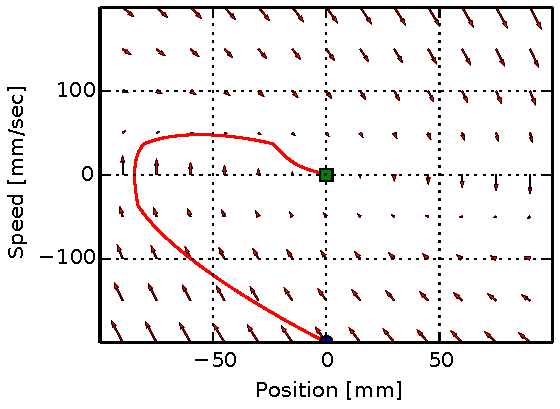
\includegraphics[width=0.32\textwidth]{ppq.pdf}
				\label{fig:phase_plane_LQR}}
				\subfloat[Minimum energy]{
				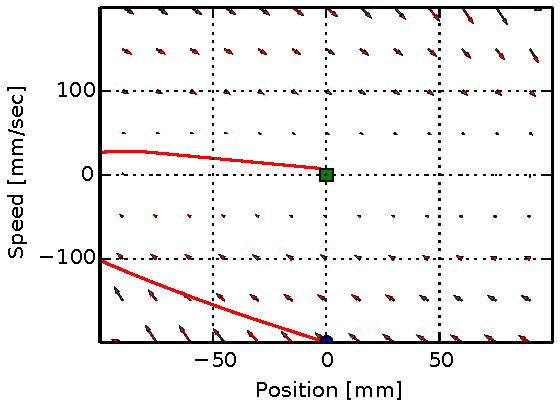
\includegraphics[width=0.32\textwidth]{ppe.pdf}
				\label{fig:phase_plane_energy}}
        \caption{Closed loop behavior with the optimal policy illustrated in the phase plane}\label{fig:phase_plane}
\end{figure}

\subsection{Reinforcement Learning}



\section{Simulation Results}
\label{sec:shift_sim}

TODO


\section{Experiments Results}
\label{sec:shift_exp}

\subsection{Dynamic motions}
\label{sec:DynamicMotions}


Here a trajectory following experiments using the last DoF of the robot only is presented. A 1.5 Kg load is mounted on the end-effector, and the task is to bring it from the bottom position ($q=-\pi$) to the up-right position ($q=0$) using as little torques as possible. An RRT trajectory planning algorithm is used to search for a low torque trajectory reaching the goal, see Fig. \ref{fig:exp_rrt}. Then the R* Computed Torque Controller is used to track the reference trajectory. The experimental results are shown in Fig. \ref{fig:exp_traj} and a video of this experiment is also available in the multimedia attachment. 
%
\begin{figure}[htp]
	\centering
		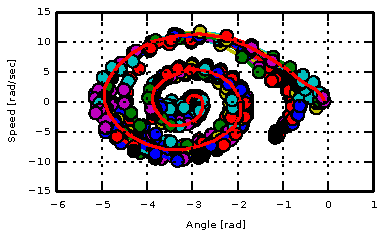
\includegraphics[width=0.75\textwidth]{rrt_fig.pdf}
	\caption{Trajectory generation algorithm searching for a low torque solution}
	\label{fig:exp_rrt}
\end{figure}
%
\begin{figure}[htp]
	\centering
		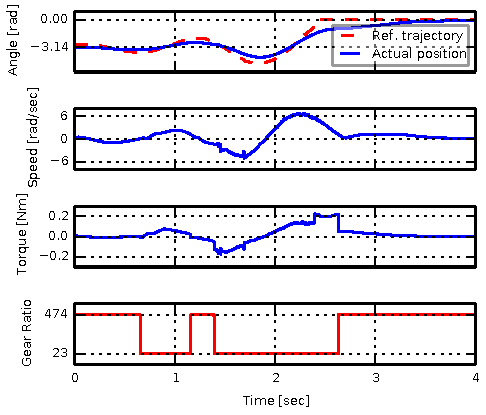
\includegraphics[width=0.75\textwidth]{exp_fig3.pdf}
	\caption{Experimental results}
	\label{fig:exp_traj}
	\vspace{-10pt}
\end{figure}
%
Results show that the robot is using its 1:23 gear-ratio to accumulate kinetic energy by swinging the arm link back and forth. Also the R* controller selects the 1:474 gear-ratio automatically to attenuate the load dynamics, when the actuator has to force the robot to stay with the trajectory.  Interestingly, the reference trajectory was planned so the robot would accumulate enough kinetic energy to swing straight up with the last swing. However, in the experiment, the dissipative forces are greater than anticipated by the planner, and the last swing is too small (the robot almost stop at $q=-0.9$ at $t=2.6$ in Fig. \ref{fig:exp_traj}). Then, the R* controller automatically engage the large 1:474 gear-ratio, to continue converging on the desired trajectory with much smaller torques than those required if keeping using the 1:23 gear-ratio in this situation (no momentum and a large gravitational force to overpower). This illustrates that including the gear-ratio selection in the feedback loop also increase the robustness of the system. Without the 1:474 gear-ratio option, tracking would have failed as the computed torque with 1:23 in this situation was greater than the maximum allowable motor torque.
